\documentclass[a4paper,onesided,12pt]{report}
\usepackage{styles/fbe_tez}
\usepackage[utf8x]{inputenc} % To use Unicode (e.g. Turkish) characters
\renewcommand{\labelenumi}{(\roman{enumi})}
\usepackage{amsmath, amsthm, amssymb}
 % Some extra symbols
\usepackage[bottom]{footmisc}
\usepackage{cite}
\usepackage{graphicx}
\usepackage{longtable}
\graphicspath{{figures/}} % Graphics will be here

\usepackage{multirow}
\usepackage{subfigure}
\usepackage{algorithm}
\usepackage{algorithmic}
%\pagestyle{empty}
%\includeonly{introduction} % To only process the given file

\newtheorem{thm}{Theorem}[chapter]
\newtheorem{prop}[thm]{Proposition}
\newtheorem{lem}[thm]{Lemma}
\newtheorem{cor}[thm]{Corollary}
% COVER PAGE
\title{Gate Level Event-Driven Simulation using GPGPUs with CUDA}
%\degree{Senior, in Computer Engineering, Boğaziçi University, 2012}
\degree{\ }
\author{Seçkin Savaşçı}
\program{Computer Engineering}
\subyear{2012}

% APPROVED BY PAGE
\supervisor{Prof. Alper Şen}
%\cosuperi{Title and Name of Cosupervisor I}
%\cosuperii{Title and Name of Cosupervisor II}
%\examineri{Assoc. Prof. Name Surname}
%\examinerii{Assist. Prof. Name Surname}
%\examineriii{Name Surname, Ph.D.}
%\examineriv{}
%\examinerv{}
\dateofapproval{\ }

\begin{document}

\pagenumbering{roman}
\makebstitle % B.S. thesis
\makeapprovalpage
%\begin{acknowledgements}
%Acknowledgements come here...
%\end{acknowledgements}
%\begin{abstract}
%One page abstract will come here.  
%\end{abstract}

\tableofcontents
\newpage

\chapter{Abstract}
\label{chapter:Abstract}
\pagenumbering{arabic}
 A typical digital design flow starts with creating an architectural model. Then designers convert this model into an HDL level design such as RTL model. VHDL or Verilog can be used for this step. After it, a synthesis tool synthesize structural gate level netlist consisting logic primitives. Finally this netlist is implemented on a silicon chip. If the prototype chips work as intended, then they will be released and used in end-user systems.
 
  
 However more than half of the effort in the design phase goes for verification and validation of the design, which is known as pre-silicon verification. In RTL level, validation is easier to do with extensive tool support. On the other hand, netlist validation(functional validation) is mainly done by simulation. Performance for gate level netlist simulation is extremely low; typically it takes days to validate a particular design. But netlist simulation performance is quite significant since short times-to-market limit the coverage that can be achieved in verification. Thus, faster verification methods are needed to improve coverage. Any improvement in any phase of the validation can improve the overall performance of the validation flow. In this context, GPGPUs can deliver faster gate level simulation by exploiting the parallelism. 
 
 
 As the senior project, it is given to implement event-driven gate level simulation on GPGPUs using CUDA. Having little experience on event-driven simulation, digital design implementation and CUDA makes the project a self-learning task as well as an implementation task.Project is subdivided into the learning and implementation tasks. Even if the learning and implementation tasks can be interleaved to some extent, it is chosen to minimize interleaving of them to avoid major design problems and wrong costly decisions since the student is new to this field. To complete the learning task and to start to the implementation, the student must:
 \begin{itemize}
 \item learn and practice CUDA, 
 \item review core digital design topics including logic components,
 \item review core simulation topics with special focus on event-driven simulation,
 \item learn how event-driven simulation is applied in logic level circuitry. 
 \end{itemize} 
 
 We come up with a parallel circuit simulator which runs up to 6 times faster comparing to its sequential equivalent. Our main contributions are:
 \begin{itemize}
 \item \textbf{Circuit Generator} \\ A random circuit generator for our own circuit format
 \item \textbf{Run Generator} \\ A random run generator that feeds the simulation with inputs in each timestep
 \item \textbf{Sequential Event-Driven Circuit Simulator(Enigma)} \\ A sequential circuit simulator written in C++
 \item \textbf{Parallel Event-Driven Circuit Simulator(Meepo)} \\ Our project goal, parallelized version of Enigma simulator, 
 with the help of CUDA
 \end{itemize}
 
 \chapter{Introduction}
 \section{Learning and Practicing CUDA}
 
 CUDA stands for \emph{Compute Unified Device Architecture}. It is a parallel programming platform and a programming model created by NVIDIA. It enables programmers to develop programs using massively parallel architecture of GPUs.
 
 Not surprisingly, GPU programming didn't start with CUDA. Computer graphics developers were(and still they are) programming for GPUs using so-called shader languages such as GLSL\footnote{http://www.opengl.org/documentation/glsl/}. The main problem in this approach is that shading languages reside natively in the computer graphics domain.So anyone interested in GPU programming must have learnt at least some computer graphics terminology before developing programs that run on GPU. CUDA solved this problem by presenting a domain agnostic way to program GPUs. CUDA offers a subset of C language and some additional identifiers like \emph{\_\_device\_\_} to solve any programming task that requires parallelism. It doesn't require any more than mediocre development experience in a C-like language. Currently all GPUs of NVIDIA on the market supports CUDA. Since these GPUs have quite different specifications and they come to market in different times, CUDA feature capabilities are rated by an index called \emph{CUDA Compute Capability}. For example, devices with Compute Capability 2.0 supports atomic floating point operations. CUDA is stil under development, currently version 5.0 is released which presents a subset of C++ class capabilities for GPU computing. 
 
 CUDA has several advantages over traditional general-purpose computation on GPUs (GPGPU) using graphics APIs:
 \begin{itemize}
 \item \textbf{Scattered reads}, code can read from arbitrary addresses in memory
 \item \textbf{Shared memory}, CUDA exposes a fast shared memory region (up to 48KB per Multi-Processor) that can be shared amongst threads. This can be used as a user-managed cache, enabling higher bandwidth than is possible using texture lookups.
 \item Faster downloads and readbacks to and from the GPU
 \item Full support for integer and bitwise operations, including integer texture lookups
 \end{itemize}
 But it also has disadvantages to consider:
 \begin{itemize}
 \item Texture rendering is not supported (CUDA 3.2 and up addresses this by introducing "surface writes" to CUDA arrays, the underlying opaque data structure).
 \item Copying between host and device memory may incur a performance hit due to system bus bandwidth and latency (this can be partly alleviated with asynchronous memory transfers, handled by the GPU's DMA engine)
 \item Threads should be running in groups of at least 32 for best performance, with total number of threads numbering in the thousands. Branches in the program code do not impact performance significantly, provided that each of 32 threads takes the same execution path; the SIMD execution model becomes a significant limitation for any inherently divergent task.
 \item Unlike OpenCL(an alternative to CUDA), CUDA-enabled GPUs are only available from Nvidia
 \item Valid C/C++ may sometimes be flagged and prevent compilation due to optimization techniques the compiler is required to employ to use limited resources.
 \item Double precision (CUDA compute capability 1.3 and above) deviate from the IEEE 754 standard: round-to-nearest-even is the only supported rounding mode for reciprocal, division, and square root. In single precision, denormals and signalling NaNs are not supported; only two IEEE rounding modes are supported (chop and round-to-nearest even), and those are specified on a per-instruction basis rather than in a control word; and the precision of division/square root is slightly lower than single precision.
 \end{itemize}
 
 Since I'm quite experienced with C language, I started learning CUDA as soon as the project overview is presented. For learning CUDA, I started reading and completed the book \emph{CUDA by Example}\cite{cuda_be} in two weeks. The book is structured in a way that each chapter covers a fundamental feature of CUDA in addition to many core concepts of parallel computing. I implemented the examples presented in the book rather than merely reading the text to get even more familiar and fast with CUDA programming.In addition to this book, I watched the webinars in CUDA Learning Zone in NVIDIA website\footnote{https://developer.nvidia.com/gpu-computing-webinars}. These webinars offer a jump-start point for developers with past experience on sequential computing.
 
 \section{Revision of Digital Design Topics}
 
 Computer Engineering Undergraduate Program in Bogazici University contains a compulsory digital design course in sophomore year, namely CMPE240 Digital Systems. The textbook of this course \emph{Frank Vahid, Digital Design, Wiley, 2011.} was a solid source of information for me at the time that I'd taken the course.
 
 To revise digital design topics, I've read very first chapters of the book and solved some of the exercises at the end of each chapter. In time, I've further consulted the book in future when I needed more information about digital design and logic components. To indicate specifically, a future student or researcher with the same topic of this project must cover \emph{hazards} and related topics essentially to excel in gate level simulation.
 
 \section{Revision of Simulation Topics}
 
 Computer engineering curriculum contains a system simulation course from industrial engineering department, namely IE306 Systems Simulation. The course aims to make students familiar with simulation systems with different approaches, indicating pros and cons of each of the techniques. Mainly discrete event simulation is taught and practiced in projects of IE306, so it suits my intentions.
 
 To review simulation topics, I consulted presentations available in the course website. They cover fundamentals of simulation topics in a paced manner. Yet it makes no more than an introduction to simulation systems. Extensive knowledge from past courses could be very beneficial for a similar project. 
 
 \section{Learning Event-Driven Simulation in Gate Level}
 
 For this learning task, the professor guided me to Peter.M.Maurer\footnote{http://cs.ecs.baylor.edu/$\sim$maurer}'s unpublished chapters on Design Automation: Logic Simulation. Chapters of the book covers simulation concepts and target common issues:
 \begin{itemize}
 \item A Review of logic design
 \item Levelized simulation
 \item Event-driven simulation
 \item Multi-delay simulation
 \item The PC-Set method
 \item The Parallel Technique
 \item The Inversion Algorithm
 \end{itemize} 
 
 Starting from levelized simulation, it presents event driven simulation in gate level with various techniques such as shadow algorithm. It touches implementation of delay in logic simulation, also gives extensible information about simulation in parallel.
 
 \chapter{Gate Level Simulation}
 \label{chapter:gate-level-simulation}
 
 Simulating individual AND, OR, and NOT gates is simple. First of all, allocate an integer for each net. Then keep the value of the net in the low-order bit of the integer. Finally, use bit-level AND, OR and NOT operators to perform the simulations. This method can be extended to networks of gates, but some care is necessary for handling memory components. Yet, the strategy here is to simulate every gate for every time-step. This is wasteful because if the inputs of a gate don't change, then the output doesn't change, either.Avoiding simulating those gates whose inputs do not change can result in improvements in terms of speed. However, a very straight-forward approach of continuously checking if the inputs are changed or not for each of the gates, will not help, since testing the inputs presents additional workload to the simulation of a gate. 
 
 Event-Driven Simulation is purposed to eliminate unnecessary gate simulations
 without introducing an unacceptable amount of additional testing. It is based on the idea of an event, which is a change in the value of a net. In a typical event driven simulation, each events are represented as a data structure,
 and these data structures acts as a trigger for simulation of gates and  creation of other events.
 
 During simulation, events trigger gate simulations and gate simulations produce
 events. If there is no new events then no gates will be simulated. The initial set of events is created by comparing each bit of an input vector with the corresponding bit in the previous input vector. An event is created for each pair of bits that is different. Thereafter, nets are tested for changes only after a gate simulation. When an event is processed, any gates that use the net as an input will be scheduled for simulation. The order in which gate simulations are performed cannot be predicted ahead of time, so dynamic queues are used to schedule both event processing and gate simulation. When an event is detected, an event structure will be created and stored in the \emph{Event
 Queue} for future processing. Event processing continues until all events have been processed and removed from the \emph{Event Queue}. At this point, there will usually be several gates in the \emph{Gate Queue}. Then gates in gate queue are simulated, tested their outputs for changes, and schedule events. An alternative approach is to eliminate the gate queue or the event queue and use a single scheduling queue. Such an approach is called Single-List or One-List scheduling to contrast it with Two-List scheduling. Both of the strategies comes with gains and drawbacks in several aspects. Event-driven simulation presents by default a unit delay timing strategy yet multi-delay strategies can be adopted by using techniques like time wheel. In our final deliverable, multi-delay timing is adopted and we've implemented Two-List queuing strategy.
 
 
   
 
 \chapter{Related Work on Gate Level Simulation}
 \label{chapter:related-work}
 
Research on logic simulators gain importance and interest when the
concepts of circuit netlist compilation, oblivious and event-driven
simulation were first discovered. Particularly,Baker et al.\cite{baker} provide
an analysis of early attempts to parallelize event-driven
simulation by dividing the processing of individual events
across multiple machines with fine granularity. But fine granularity
comes with a high communication overhead and, depending
on the solution, the issue of deadlock avoidance needs sophisticated
event handling. There are also parallel algorithms for event-driven simulation
for distributed systems \cite{manjikian,matsumoto} and multiprocessors
\cite{kim}. In these solutions, threads run on separate netlist clusters and communication is done with an event-driven fashion.  

Today, several commercial simulators building on these concepts
are available: they execute on a single CPU and adopt aggressive
compiled-code optimization techniques to boost their performance.
In addition, specialized hardware solutions (emulation systems)
have also been implemented to boost simulation performance.
 Modern emulators can deliver 3-4 orders of magnitude
speedup and they can handle very large designs. However, their
cost is high and the process of successfully mapping
a netlist to an emulator can take up to few months.
Most recently, a few research solutions have been presented to
run simulations on GPUs: an early attempt by Perinkulam et al.\cite{perinkulam} fail to satisfy because of not providing performance benefits due to lack of general purpose
programming primitives (CUDA like language, data transfer overhead etc.) for their platform and the high communication
overhead. An oblivious simulator solution can be seen in the work of Bertasco et al \cite{bertasco}.Yet expectedly, the size of the circuits that can be simulated with the solution in \cite{bertasco} is severely limited by the size of the shared memory in the GPU platform.
Chatterjee et al\cite{chatterjee} introduce macro-gate concept and proposes a solution which targets fast simulation of complex designs which circuit partitioning and optimizations techniques in order to enhance the parallelism of the target platform. Şen et al\cite{sen} provides a similar Cycle-based simulation solution to \cite{chatterjee} yet using And-Inverter Graphs.

\chapter{Contributions}
\label{chapter:contributions}
 
\section{Circuit Generator}
To test the simulators, we should come up with input circuits. In that time, we had two options: Either we collect existing popular circuits on simulation research area or we implement a circuit generator. In order to focus more on implementing the simulators, we choosed the easier way: Implementing a random circuit generator with a simple format. With circuit generator which comes with the final deliverable and written in C++, one can easily generate random circuits by specifying number of gates, number of inputs, number of outputs. We choosed to give .cir extension to circuit files. The exact call syntax is:
\begin{verbatim}
./circuit_generator <num_gates> <num_inputs> <num_outputs> <circuit_filename>
\end{verbatim} 
After this call, a random circuit is generated with a simple format such that:
\begin{verbatim}
<num_gates> <num_nets>
<num_inputs> <list_of_inputs>
<num_outputs> <list_of_outputs>
<gate_type> <input_netID_1> <input_netID_2> <output_netID> <delay>
<gate_type> <input_netID_1> <input_netID_2> <output_netID> <delay>
  ...
 \end{verbatim}
 
 
 \section{Run Generator}
 
 To feed the simulators with input vectors in each timestep, we also implement a run generator which randomly generates input vectors for a given timestep amount. The exact call syntax is:
 \begin{verbatim}
 run_generator <circuit_file> <num_runs> <run_filename>
 \end{verbatim}
 As anyone can notice, run generator autmatically investigates the circuit file and create random input vectors according to that. The output file which by out tradition has extension .run and only contains input vectors in each timestep such format:
\begin{verbatim}
<in0> <in1> ..... <inN>
<in0> <in1  ..... <inN>
\end{verbatim}

 \section{Overall Structure of Simulation}
 In this work, multi-delay two-list simulation is used. In two-list simulation, there are two processors and two queues. When a net value change is to happen a corresponding event is generated. This event generation can be triggered by either a change in respective input or a change in gate output in previous timestep. At first, this event queue is passed to event processor, event proccessor process each event that is scheduled for the current timestep such that:
 \begin{itemize}
 \item change indicated nets value by the value in event data
 \item investigate fanout of this net and schedule this gates to be simulated by pushing them in gate queue.
 \end{itemize} 
 
 After event processor processes all events which are scheduled for current timestep, we have possibly non-zero size gate queue. This gate queue stores the gates which is need to be simulated for current time step. Like in event processing, this gate queue is forwarded to gate processor. Gate processor's workflow is:
 \begin{itemize}
 \item Simulate the given gate
 \item If output is changed, then create an event for output net and push it to event queue
 \end{itemize}
 
 \begin{figure}[htbp]
 		\centering
 		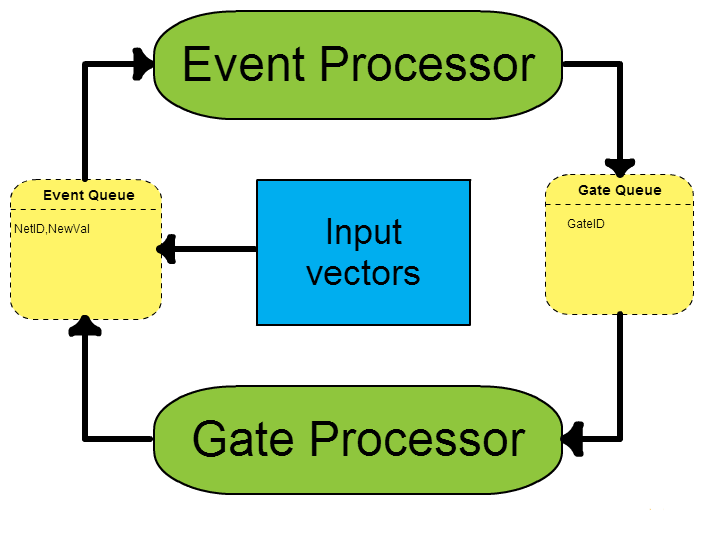
\includegraphics[height=0.30\textheight]{diagram.png}
 		\caption{Overall Simulation Logic}
 \end{figure}
 
 Let's make it demonstrate with a simple demo circuit! \\
 We have a circuit which specified in demo1.cir and corresponding input vectors are generated in demo1.run. demo1.cir contains:
 \begin{verbatim}
 6 12
 6 0 1 2 3 4 5
 3 9 10 11
 0 0 1 6 1
 0 2 3 7 1
 0 4 5 8 1
 1 6 7 9 1
 1 7 8 10 1
 2 9 9 11 1
 \end{verbatim}
 To interpret this file; demo1 circuit contains 6 gates and 12 nets, inputs are 0 1 2 3 4 and 5 and we have 3 outputs which are net 9 10 and 11. Then gate description starts: We have type0(AND) gate which is connected to net0 and net1 as inputs and net6 to output, it has unit delay. The other five gates are interpreted similarly. ( type1 represents OR gate and type2 represents NOT gate)

  \begin{figure}[htbp]
  		\centering
  		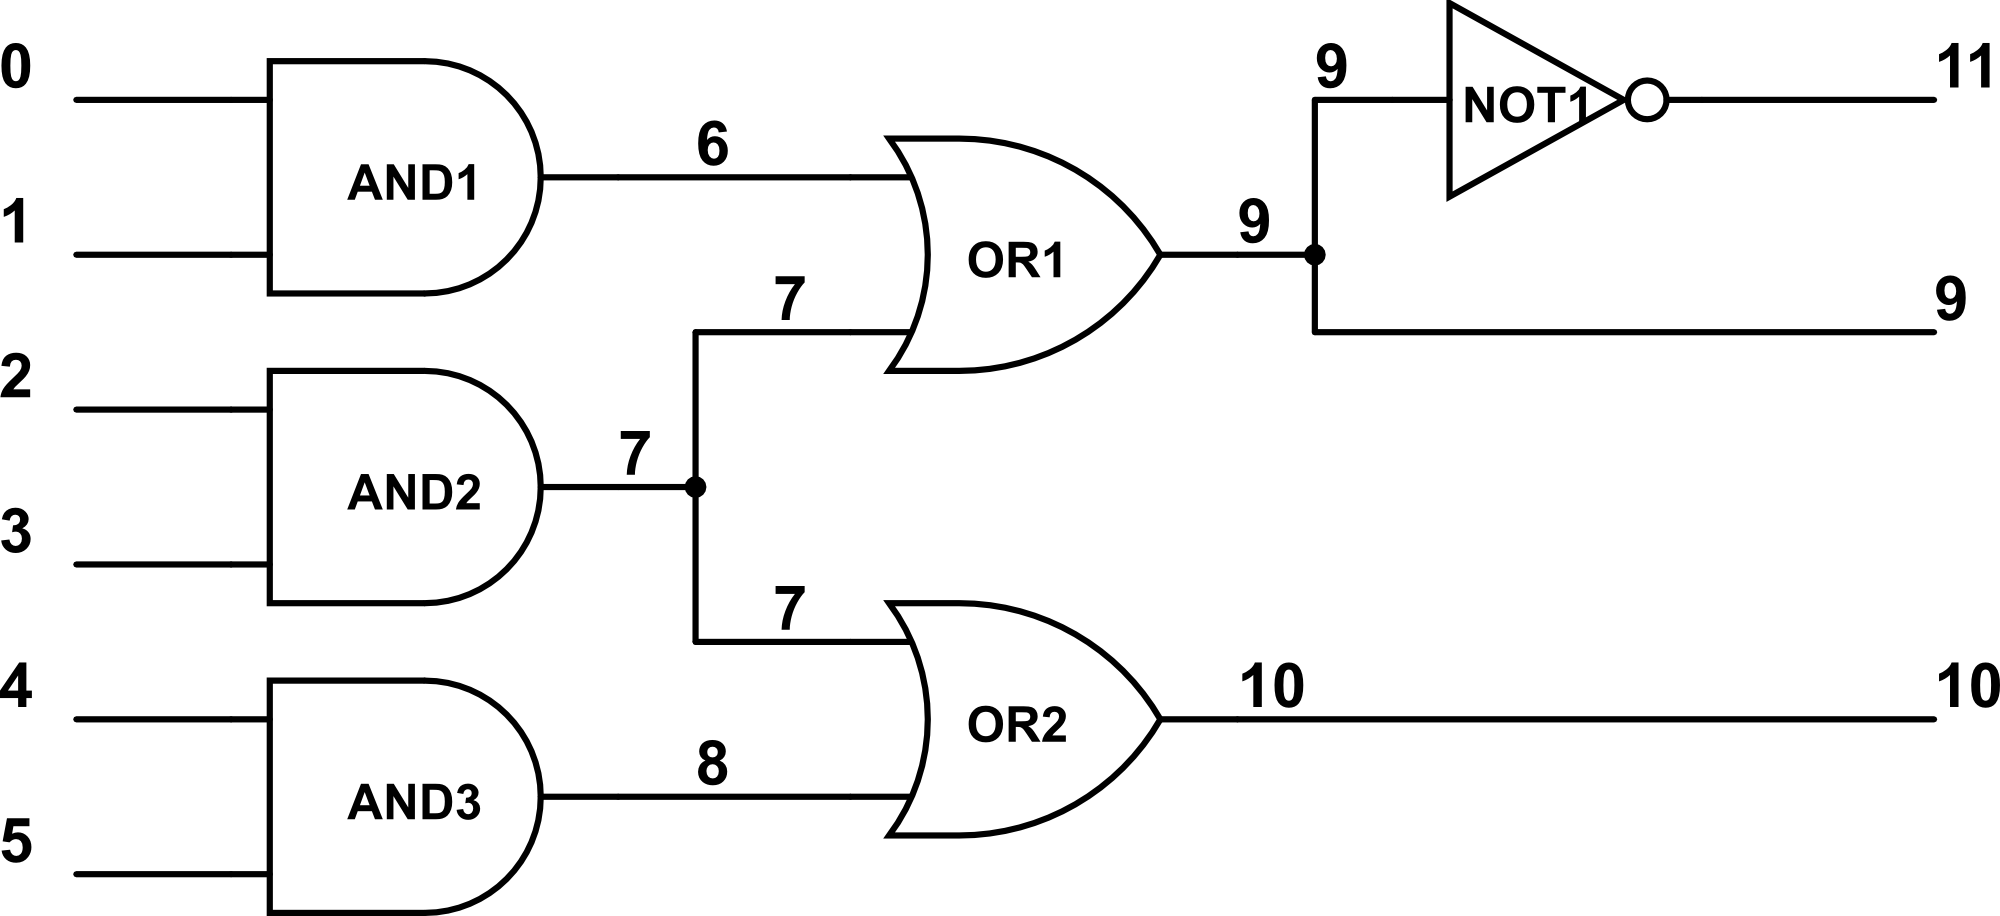
\includegraphics[height=0.25\textheight]{senior_demo.png}
  		\caption{Representation of circuit in demo1.cir}
  \end{figure}
 In the other hand, our demo1.run is:
 \begin{verbatim}
 0 0 0 0 0 0
 0 0 0 0 0 1
 0 0 0 0 1 1
 \end{verbatim}
 Order in demo1.run file is the same order of netIDs in the input declaration line of demo1.cir. \\
 In the beginning of the simulation, first input vector from demo1.run is read, and since it is the first timestep we schedule 6 events, one for each of the input nets. Event processor takes those events, change net values corresponding to the input vector and schedules gates in fanout of these nets, namely AND0, AND1, AND2 is scheduled. Gate processor gets gate queue and simulates each gate. We use tristate logic (0,1,Undef), and by default nets are set to Undef. So when the gates are simulated all 3 output gates are needed to be 0 now, and to realize this situation, 3 events for net6,net7, and net8 is created and pushed to the event queue. Before stepping to next timestep, we read the input vector again, and compare with the old vector, as you see only net5 value has changed and we create a corresponding event. Now 4 events of net5,net6,net7,net8 is sent to event processor, and as a result OR1, OR2, and AND3 gates are scheduled. Gate processors simulates this gates and schedule events for net9, net10. See that event if AND3 gate is simulated, its output didn't change even if its input has changed. Not changing the output avoid us to schedule unnecessary events.  But in the next timestep we will schedule AND3 gate again and simulation will continue to its fanouts since it will change its output to 1 in timestep 2.
 
\section{Enigma Module: Sequential Approach}
Enigma module is a sequential event-driven circuit simulator written in C++ . Concepts so far discussed are applied to this simulator. It works event-driven while processing events in gates with the corresponding orders in event and gate queue.

\section{Meepo Module: Parallel Approach}
Meepe module is a parallel event-driven circuit simulator written mainly in C++. Parallelization is achieved by using CUDA. In Meepo unlike Enigma, we've spawn one thread per gate or event. And Simulate events and gates in parallel by running these threads concurrently. We run at least 512 threads for each event processing or gate processing task. If event or gate is larger than 512, additional threads are scheduled and started immediately.
\chapter{Results}
In our tests, we simulated circuits which contain 1000, 2000, 3000, 5000, 10000, 20000, 30000. Bigger gates are omitted since one of the bigger circuit's simulation takes more than 15 minutes in Enigma module Results show that we have up to 6 times performance gain with the minumum of 2 times in the smallest circuit. Trend is that 6 times speed-up is stabilized for further simulations with bigger circuits.

\centering \begin{tabular}{| r | r | r | r |}

\hline                        
Gates & Enigma(sec) & Meepo(sec) & Speed-up \\ \hline 
1000 & 2.08 & 0.943 & 2.206 \\ \hline
2000 & 6.053 & 1.658  & 3.651 \\ \hline
3000 & 12.438 & 2.915 & 4.267 \\ \hline
5000 & 32.246 & 6.363  & 5.068 \\ \hline
10000 & 118.059 & 20.907 & 5.647 \\ \hline
20000 & 493.285 & 85  & 5.803 \\ \hline
30000 & 1060.34 & 181.785  & 5.833 \\ \hline
\end{tabular}


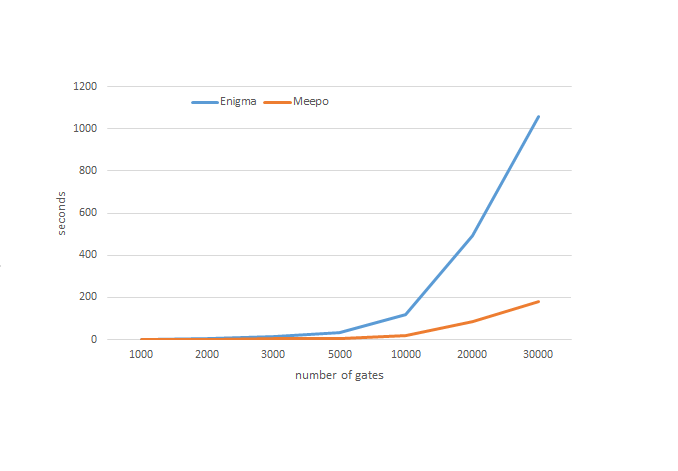
\includegraphics[height=0.45\textheight]{graph1.png} 
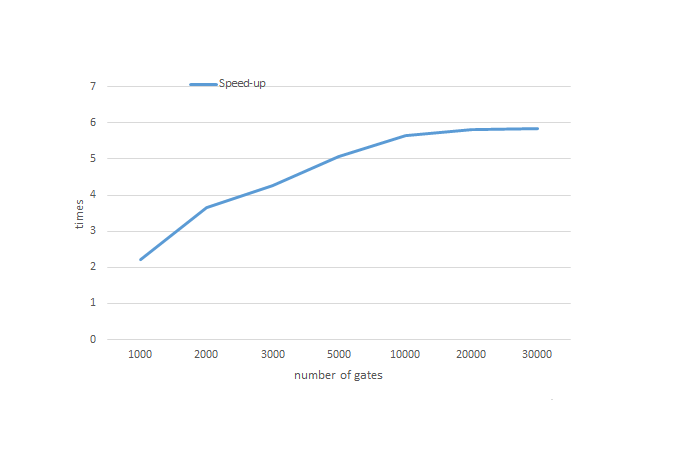
\includegraphics[height=0.45\textheight]{graph2.png} 

\chapter{Conclusion}

This project was a good opportunity to learn and apply event-driven gate simulation and parallel programming. It can also be given as a year long senior project with some extensions. I'm satisfied with the results yet more can be done to increase performance. I have written that report in order to help a future reader to understand our work and build on top of our achievements.

I want to thank you my project advisor Alper Şen for his great helps especially in learning stage. I wouldn't complete this project without the resources  he'd provided.

\appendix

%\cite{*}
\bibliographystyle{styles/fbe_tez_v11}
\bibliography{references}

\chapter{Source Code : Circuit Generator}
\section{circuit.h}
\tiny \begin{verbatim} 
#ifndef CIRCUIT_H
#define CIRCUIT_H

enum { AND, OR, NOT, NAND, NOR, XNOR, FLIPFLOP };

struct Gate{
int type;
int in1;
int in2;
int out;
int delay;
};

class Circuit
{
public:
	int num_gates;
	int num_nets;
	int num_inputs;
	int num_outputs;
	struct Gate* gates;

};

#endif
\end{verbatim}

 \section{main.cpp}
 \begin{verbatim}
 #include <iostream>
 #include <fstream>
 #include <time.h>
 #include "circuit.h"
 #include <vector>
 #include <algorithm>
 using namespace std;
 
 int main(int argc,char ** argv)
 {
 	cout << "Generating circuit.." << endl;
 	srand(time(NULL));
 	int num_types,max_delay,current_net_count;
 
 
 	Circuit circ;
 
 	num_types = 3;
 	max_delay = 5;
 	circ.num_gates=atoi(argv[1]);
 	circ.num_nets=0;
 	circ.num_inputs=atoi(argv[2]);
 	circ.num_outputs = atoi(argv[3]);
 	current_net_count = circ.num_inputs;
 	circ.gates = new struct Gate[circ.num_gates];
 
 	for(int i=0;i<circ.num_gates;i++)
 	{
 		circ.gates[i].type = rand() % num_types; 
 		circ.gates[i].in1=-1;
 		circ.gates[i].in2=-1;
 		circ.gates[i].out=-1;
 		circ.gates[i].delay= (rand() % (max_delay+1))+ 1;
 	}
 	int selection;
 	for(int i=0;i<circ.num_inputs;i++)
 	{
 randomize:	selection = rand() % circ.num_gates;
 		if(circ.gates[selection].in1 == -1 ) circ.gates[selection].in1 = i;
 		else if(circ.gates[selection].in2 == -1 ) circ.gates[selection].in2 = i;
 		else goto randomize;
 	}
 
 	for(int i=0;i<circ.num_gates;i++)
 	{
 		circ.gates[i].out = current_net_count;
 		current_net_count++;
 
 		if(circ.gates[i].type == NOT )
 		{
 			do{
 
 				if(circ.gates[i].in1 != -1 && circ.gates[i].out != circ.gates[i].in1) circ.gates[i].in2 = circ.gates[i].in1;
 				else if(circ.gates[i].in2 != -1 && circ.gates[i].out != circ.gates[i].in2) circ.gates[i].in1 = circ.gates[i].in2;
 				else 
 				{
 					circ.gates[i].in1 = rand() % current_net_count;
 					circ.gates[i].in2 = circ.gates[i].in1;
 					//current_net_count++;
 				}
 			}while(circ.gates[i].in1 == circ.gates[i].out);
 		}
 		else
 		{
 			if(circ.gates[i].in1 ==-1) 
 			{
 				do
 				{
 					circ.gates[i].in1 =rand() % current_net_count;
 				}while(  circ.gates[i].in1 == circ.gates[i].out);
 				//current_net_count++;
 			}
 			if(circ.gates[i].in2 ==-1) 
 			{
 				do
 				{
 					circ.gates[i].in2 = rand() % current_net_count;
 				}while(circ.gates[i].in2 == circ.gates[i].in1 || circ.gates[i].in2 == circ.gates[i].out);
 				//current_net_count++;
 			}
 		}
 
 	}
 
 	/*for(int i=0;i<circ.num_gates;i++)
 	{
 		circ.gates[i].out = (rand() % (current_net_count-circ.num_inputs))+ circ.num_inputs;
 	}*/
 
 	circ.num_nets = current_net_count;
 	ofstream outFile(argv[4]);
 	outFile << circ.num_gates << " " << circ.num_nets << endl;
 	outFile << circ.num_inputs << " " ;
 	for(int i=0;i<circ.num_inputs;i++) outFile << i << " ";
 	outFile << endl;
 	outFile << circ.num_outputs << " ";
 
 	vector<int> outputs;
 	
 	for(int i=0;i<circ.num_outputs;i++) outputs.push_back( (rand() % (circ.num_nets - circ.num_inputs))+ circ.num_inputs );
 	sort(outputs.begin(),outputs.end());
 
 	for(int i=0;i<circ.num_outputs;i++) outFile << outputs[i] << " ";
 	outFile << endl;
 	for(int i=0;i<circ.num_gates;i++)
 	{
 		outFile << circ.gates[i].type << " "; 
 		outFile << circ.gates[i].in1  << " ";
 		outFile << circ.gates[i].in2  << " ";
 		outFile << circ.gates[i].out  << " ";
 		outFile << circ.gates[i].delay << " ";
 		outFile << endl;
 	}
 	cout << "Circuit generated!" << endl;
 	cout << "Gates : " << circ.num_gates << endl;
 	cout << "Inputs : " << circ.num_inputs << endl;
 	cout << "Outputs : " << circ.num_outputs << endl;
 }
 \end{verbatim}

\chapter{Source Code : Run Generator}
\section{main.cpp}
\begin{verbatim}
#include <iostream>
#include <fstream>
#include <time.h>

using namespace std;

int main(int argc,char** argv)
{
	int num_gates,num_nets,num_inputs,num_runs;
	ifstream inFile(argv[1]);
	ofstream outFile(argv[3]);
	num_runs= atoi(argv[2]);
	srand(time(NULL));

	inFile >> num_gates >> num_nets >> num_inputs;

	cout << "Gates : " << num_gates << " Nets : " << num_nets << " Inputs : " << num_inputs << endl;
	cout << "Generating simulation run..." << endl;

	for(int i=0 ;i<num_runs;i++)
	{
		for(int j=0;j<num_inputs;j++)
		{
			outFile << (rand() % 2) << " ";
		}
		outFile << endl;
	}
	cout << argv[3] << " run file generated successfully" << endl;
	return 0;
	
}
\end{verbatim}

\chapter{Source Code : Enigma(Sequential) Module}
\section{circuit.h}
\begin{verbatim}
#ifndef CIRCUIT_H
#define CIRCUIT_H

#include "gate.h"
#include "net.h"

class Circuit
{
public:
	int fanwide;
	int num_gates;
	int num_nets;
	int num_inputs;
	int num_outputs;
	int* outputs;
	int* inputs;
	Gate* gates;
	char* nets;
	int* fanouts;
	int* gatefanouts;


	Circuit(char * filename);
	~Circuit();
	void printNets();
	void printFanouts();
	void printGates();
};

#endif
\end{verbatim}
\section{circuit.cpp}
\begin{verbatim}
#include <iostream>
#include <fstream>
#include "circuit.h"



using namespace std;



Circuit::Circuit(char* filename)
{
	//Process decleration
	cout << "Parsing circuit description from..." << endl;
	cout << "... " << filename << endl;

	//Initial read
	std::ifstream inFile(filename);
	inFile >> this->num_gates >> this->num_nets;
	cout << "Circuit contains " << this->num_gates << " gates."<< endl;
	
	this->gates = new Gate[num_gates];
	this->nets = new  char[num_nets];

	for(int i=0;i<num_nets;i++)
	{
		nets[i]=-1;
	}
	
	inFile >> this->num_inputs;
	cout << "Input vector size in each pass : " << this->num_inputs << endl;
	
	this->inputs = new int[num_inputs];

	
	
	fanwide = (100>(num_gates/10+5))?(num_gates/10+5):(100);
	fanouts = new int[num_nets*fanwide];
	for(int i=0;i< num_nets*fanwide;i++)
	{
		fanouts[i] = -1;
	}

	cout << "Reading input IDs" << endl;
	for(int i=0;i<num_inputs;i++)
	{
		inFile >> inputs[i];
	}
	cout << "Input IDs: " ;
	for(int i=0;i<num_inputs;i++)
	{
		cout << inputs[i] << " ";
	}
	cout << endl;

	inFile >> this->num_outputs;
	cout << "Output vector size in each pass : " << this->num_outputs << endl;

	this->outputs = new int[num_outputs];

	cout << "Reading output IDs" << endl;
	for(int i=0;i<num_outputs;i++)
	{
		inFile >> outputs[i];
	}
	cout << "Output IDs: " ;
	for(int i=0;i<num_outputs;i++)
	{
		cout << outputs[i] << " ";
	}
	cout << endl;

	cout << "Listing gates:"<< endl;
	int type,delay;
	for(int i=0;i<num_gates;i++)
	{
		inFile >> type >> gates[i].in[0] >> gates[i].in[1] >> gates[i].out >> delay;
		gates[i].type = type;
		gates[i].delay = delay;
		gates[i].val=-1;
		
		for(int j=0 ; j< fanwide ;j++)
		{
			if(fanouts[gates[i].in[0]*fanwide+j] == i) break;
			if(fanouts[gates[i].in[0]*fanwide+j] == -1 )
			{
					fanouts[gates[i].in[0]*fanwide+j] = i;
					break;
			}
			if(j == fanwide-1) cout << "Full, increase fanwide value." << endl;

		}

		for(int j=0 ; j< fanwide ;j++)
		{
			if(fanouts[gates[i].in[1]*fanwide+j] == i) break;
			if(fanouts[gates[i].in[1]*fanwide+j] == -1 )
			{
					fanouts[gates[i].in[1]*fanwide+j] = i;
					break;
			}
			if(j == fanwide-1) std::cout << "Full,increase fanwide value." << std::endl;

		}
		
	}
	//printGates(); //DEBUG
	// printFanouts(); //DEBUG
	
	//gatefanouts = new int[num_gates*4];
	//std::cout << "gate fanouts" << std::endl;
	//for(int i=0;i<num_gates;i++)
	//{
	//	for(int j=0;j < fanwide;j++)
	//	{
	//		//std::cout << fanouts[gates[i].out*fanwide + j] << " ";
	//		gatefanouts[i*fanwide + j] = fanouts[gates[i].out*fanwide + j];
	//	}
	//	std::cout << std::endl;
	//}
	//for(int i=0;i<num_gates;i++)
	//{
	//	for(int j=0;j < fanwide;j++)
	//	{
	//		std::cout << gatefanouts[i*fanwide+j] << " ";
	//	}
	//	std::cout << std::endl;
	//}
	
	//std::cout << nets[6].fanout[0] << std::endl;


}

void Circuit::printNets()
{
	std::cout <<"nets: ";
	for(int i=0;i<num_nets;i++)
	{
		std::cout << (int)nets[i] << " ";
	}
	std::cout << std::endl;
}

void Circuit::printFanouts()
{
	cout << "Printing fanouts: " << endl;
	for(int i=0;i<num_nets;i++)
	{
		
		cout <<"net " << i <<" : " ;
		for(int j=0;j<fanwide;j++)
		{
			if(fanouts[i*fanwide + j]== -1 && j==0)
			{
				cout << "none";
			}
			if(fanouts[i*fanwide + j]== -1) break;
			cout << fanouts[i*fanwide + j] << " ";
		}
		cout << endl;

	}
}

void Circuit::printGates()
{
	for(int i=0;i<num_gates;i++)
	{
		switch (gates[i].type)
		{
		case AND:
			cout << "AND";
			break;
		case OR:
			cout << "OR";
			break;
		case NOT:
			cout << "NOT";
			break;
		default:
			cout << "indef";
			break;
		}
		cout << "(" << i << ")" ;
		cout << " connected to nets: " << gates[i].in[0] << " , "<< gates[i].in[1] << " ; outnet: " << gates[i].out << " val="<< (int)gates[i].val<< " delay:" << (int)gates[i].delay << endl;
	}
}
\end{verbatim}
\section{event.h}
\begin{verbatim}
#ifndef EVENT_H
#define EVENT_H

class Event
{ 
public:
	int netID;
	char value;
	int time;
	Event(int ID,char val,int time);
};



#endif
\end{verbatim}
\section{event.cpp}
\begin{verbatim}
#include "event.h"

Event::Event(int ID,char val,int timeVal)
{
	netID = ID;
	value = val;
	time = timeVal;
}
\end{verbatim}

\section{gate.h}
\begin{verbatim}
#ifndef GATE_H
#define GATE_H

enum { AND, OR, NOT, NAND, NOR, XNOR, FLIPFLOP };

class Gate
{
public:
	char type;
	int  in[2];
	int out;
	char val;
	char delay;


};

#endif
\end{verbatim}
\section{main.cpp}
\begin{verbatim}
#include <iostream>
#include "simulator.h"
#include <ctime>
#include <fstream>

using namespace std;

int main()
{
	 std::cout << "Hello World!" << std::endl;
	 //Circuit* c1 = new Circuit("demo1.cir");

	 clock_t begin = clock();
	 Simulator* sim = new Simulator("./../../inputs_outputs/30000.cir","./../../inputs_outputs/30000.run","./../../inputs_outputs/30000_enigma.out");
	 clock_t end = clock();

	 double elapsed_secs = double(end - begin) / CLOCKS_PER_SEC;

	 cout << "Simulation time : " << elapsed_secs << endl;
	 cout << "Simluation steps: " << sim->timestep << endl;
	 cout << "Simulation time per timestep :" << elapsed_secs/(sim->timestep) << endl;

	 ofstream logFile;
	 logFile.open("./../../inputs_outputs/log_enigma.log",ios::out | ios::app);
	 logFile << elapsed_secs << " " <<  elapsed_secs/(sim->timestep) << endl;



	 return 0;
}
\end{verbatim}
\section{simulator.h}
\begin{verbatim}
#ifndef SIMULATOR_H
#define SIMULATOR_H
#include "circuit.h"
#include "event.h"
#include <algorithm>
#include <iostream>
#include <fstream>
#include <vector>

class Simulator
{
public:
	Circuit* circ;
	std::vector<Event> eventQueue;
	std::vector<int> gateQueue;
	int timestep;
	char* prev_val_buffer;
	Simulator(char* circuitFile,char* runFile,char* outFile);
	void processEvents();
	void processGates();
	void printEventQueue();
	void printGateQueue();
	void dumpNets(std::ofstream &offs);
	int simulateGate(int gateID);
};
#endif																								
\end{verbatim}
\section{simulator.cpp}
\begin{verbatim}
#include "simulator.h"
#include <ctime>
#include <string>
#include <iomanip>

#define OUTPUT_ONLY 1

using namespace std;

std::ostream& field(std::ostream& o)
{
    // usually the console is 80-character wide.
    // divide the line into four fields.
    return o << setw(10) << std::right;
}

Simulator::Simulator(char* circuitFile,char* runFile,char* outFile)
{
	timestep = 0;
	circ = new Circuit(circuitFile);
	std::cout << "Circuit file is read successfully!" << std::endl;
	
	std::ifstream runs(runFile);
	std::ofstream resultdump(outFile);
	resultdump << "Results for " << circuitFile << " with the trace in " <<  runFile << endl;
	dumpNets(resultdump);
	prev_val_buffer = new char[circ->num_inputs];


	//Initial Schedule
	
	cout <<"Initial Scheduling..." << endl;
	int intval;
	for(int i=0 ;i<circ->num_inputs;i++)
	{
		runs >> intval;
		prev_val_buffer[i]=intval;
		eventQueue.push_back(Event(circ->inputs[i],prev_val_buffer[i],timestep));
	}

	//printEventQueue();
	cout << "Initial Scheduling is done!" << endl;
	int current;
	clock_t begin,end;
	double elapsed_secs;

	cout << field << "Events "<< field << " Gates" <<field << "Time" << field << "Run" <<  endl;
	while(1)
	{
		begin = clock();
		//printEventQueue();// DEBUG
		cout << "\r" << field << eventQueue.size() << " ";
		processEvents();
		//circ->printNets();// DEBUG
		//printEventQueue();// DEBUG

		sort(gateQueue.begin(),gateQueue.end());
		cout << field << gateQueue.size() << " ";
		//printGateQueue();// DEBUG
		processGates();
		dumpNets(resultdump);
		timestep++;
		for(int i=0;i< circ->num_inputs;i++)
		{
			runs >> current;
			if(runs.eof()) break;
			if(prev_val_buffer[i] == current) continue;
			prev_val_buffer[i] = current;
			eventQueue.push_back(Event(circ->inputs[i],prev_val_buffer[i],timestep));
		}
		if(runs.eof() && eventQueue.size()==0 && gateQueue.size()==0 ) break;
		end = clock();
		elapsed_secs = double(end - begin) / CLOCKS_PER_SEC;
		cout << field << elapsed_secs; 
		cout << field << timestep;
		//system("PAUSE");
	}
	//printEventQueue();// DEBUG
	cout << endl;
	
}

void Simulator::dumpNets(ofstream &offs)
{

	if(OUTPUT_ONLY)
	{
		for(int i=0;i<circ->num_outputs;i++)
		{
			if( circ->nets[circ->outputs[i]] == -1) offs << "U ";
			else offs << (int)(circ->nets[circ->outputs[i]]) << " ";
		}
		
	}
	else
	{
		for(int i=0;i<circ->num_nets;i++)
		{
			if( circ->nets[i] == -1) offs << "U ";
			else offs << (int)(circ->nets[i]) << " ";
		}
	}
	offs << endl;
}

void Simulator::printEventQueue()
{
	cout << "Printing EventQueue content:" << endl;
	for(int i=0;i<eventQueue.size();i++)
	{
		cout <<"Event for net " << eventQueue[i].netID << ", val=" << (int)eventQueue[i].value  << " for t=" << eventQueue[i].time << endl;
	}
	if(!eventQueue.size()) cout << "Empty event queue" << endl;
}

void Simulator::printGateQueue()
{
	cout << "Printing GateQueue content:" << endl;
	for(int i=0;i< gateQueue.size();i++)
	{
		cout <<"Gate " << gateQueue[i] << endl;
	}
	if(!gateQueue.size()) cout << "Empty gate queue" << endl;
}



void Simulator::processEvents()
{
	for(int i=0;i < eventQueue.size();i++)
	{
		if(eventQueue[i].time == timestep)
		{
			// set new value
			circ->nets[eventQueue[i].netID] = eventQueue[i].value;

			//schedule fanout gates
			for(int j=0;j < circ->fanwide ; j++)
			{
				if(circ->fanouts[eventQueue[i].netID*circ->fanwide + j] == -1) break;
				
				if( find(gateQueue.begin(),gateQueue.end(), circ->fanouts[eventQueue[i].netID*circ->fanwide + j]) == gateQueue.end() ) 
				{
					//cout << "Gate " << circ->fanouts[eventQueue[i].netID*circ->fanwide + j] << " is scheduled" << endl; //DEBUG
					gateQueue.push_back( circ->fanouts[eventQueue[i].netID*circ->fanwide + j]);
				}
				else
				{
					//cout << "!!!Reschedule ignored for Gate " << circ->fanouts[eventQueue[i].netID*circ->fanwide + j] <<  endl; //DEBUG
				}
			}
		}
	}
	//remove_if(eventQueue.begin(),eventQueue.end(),currentEvent);
	//removing proccessed events
	while(1)
	{
		int dex=0;
		for( ;dex<eventQueue.size();dex++)
		{
			if(eventQueue[dex].time==timestep)
			{
					eventQueue.erase(eventQueue.begin()+dex);
					break;
			}
		}
		if(dex==eventQueue.size()) break;
	}
}


int Simulator::simulateGate(int gateID)
{
	int newVal;
	switch(circ->gates[gateID].type)
	{
	case AND:
		newVal = circ->nets[circ->gates[gateID].in[0]] & circ->nets[circ->gates[gateID].in[1]];
		break;
	case OR:
		newVal = circ->nets[circ->gates[gateID].in[0]] | circ->nets[circ->gates[gateID].in[1]];
		break;
	case NOT:
		newVal = (circ->nets[circ->gates[gateID].in[0]])?(0):(1);
			break;
	default:
		cout << "WARNING! indef gate encountered in simulation" << endl;
		break;
	}
	if(newVal!=circ->gates[gateID].val)
	{
		circ->gates[gateID].val = newVal;
		return newVal;
	}
	else return -1;
}

void Simulator::processGates()
{
	int simRes;
	for(int i=0;i<gateQueue.size();i++)
	{
		//TODO simulate gate
		simRes = simulateGate(gateQueue[i]);
		if(simRes!=-1)
		{
			eventQueue.push_back(Event(circ->gates[gateQueue[i]].out,simRes,timestep+circ->gates[gateQueue[i]].delay));
		}
	}
	gateQueue.clear();
}

////Initial Schedule
	//for(int i=0; i< circ->num_inputs; i++)
	//{
	//	//TODO schedule for circ->inputs[i]
	//	runs >> prev_val_buffer[i];
	//	
	//	//TODO multidelay impl
	//	//circ->nets[circ->inputs[i]].val = prev_val_buffer[i];
	//	for(int k=0;k<circ->fanwide;k++)
	//	{
	//		if( circ->fanouts[circ->inputs[i]*circ->fanwide+ k] == -1) break;
	//		std::cout << "gate scheduled: " << circ->fanouts[circ->inputs[i]*circ->fanwide + k] << " with " << prev_val_buffer[i] << std::endl;
	//		if( std::find(scheduled.begin(),scheduled.end(), circ->fanouts[circ->inputs[i]*circ->fanwide + k])!= scheduled.end() ) 
	//		{
	//			std::cout <<" already scheduled for the gate, not pushing again!" <<std::endl;
	//		}
	//		else scheduled.push_back(circ->fanouts[circ->inputs[i]*circ->fanwide + k]);
	//	}
	//}

	////Changing inputs
	//int current;
	//while(1)
	//{
	//	
	//	for(int i=0; i< circ->num_inputs; i++)
	//	{
	//		runs >> current ;
	//		//TODO multidelay impl
	//		//circ->nets[circ->inputs[i]].val = current;
	//		if(runs.eof()) break;
	//		if(prev_val_buffer[i] != current) 
	//		{
	//			for(int k=0;k<circ->fanwide;k++)
	//			{
	//				if( circ->fanouts[circ->inputs[i]*circ->fanwide + k] == -1) break;
	//				std::cout << "gate scheduled: " << circ->fanouts[circ->inputs[i]*circ->fanwide+ k] << " with " << current << std::endl;
	//				if( std::find(scheduled.begin(),scheduled.end(), circ->fanouts[circ->inputs[i]*circ->fanwide + k])!= scheduled.end() ) 
	//				{
	//					std::cout <<" already scheduled for the gate, not pushing again!" <<std::endl;
	//				}
	//				else scheduled.push_back(circ->fanouts[circ->inputs[i]*circ->fanwide + k]);

	//			}
	//			prev_val_buffer[i] = current;
	//		}
	//	}
	//	if(runs.eof()) break;

	//	circ->writeNets();
	//}

\end{verbatim}

\chapter{Source Code : Meepo (Parallel) Module}
Helper Cuda functions like HANDLE$\_$ERROR can be found in book Cuda by Example.
\section{circuit.h}
Same as in enigma, omitted here. 
\section{circuit.cpp}
Same as in enigma, omitted here.
\section{event.h}
Same as in enigma, omitted here. 
\section{event.cpp}
Same as in enigma, omitted here.
\section{gate.h}
Same as in enigma, omitted here. 
\section{gate.cpp}
Same as in enigma, omitted here.
\section{main.cpp}
\begin{verbatim}
#include <iostream>
#include "simulator.h"
#include <ctime>
#include <fstream>

using namespace std;

int main()
{
	 std::cout << "Hello World!" << std::endl;
	 //Circuit* c1 = new Circuit("demo1.cir");
	 clock_t begin = clock();
	 Simulator* sim = new Simulator("./../../inputs_outputs/30000.cir","./../../inputs_outputs/30000.run","./../../inputs_outputs/30000_meepo.out");
	 clock_t end = clock();

	 double elapsed_secs = double(end - begin) / CLOCKS_PER_SEC;

	 cout << "Simulation time : " << elapsed_secs << endl;
	 cout << "Simluation steps: " << sim->timestep << endl;
	 cout << "Simulation time per timestep :" << elapsed_secs/(sim->timestep) << endl;

	 ofstream logFile;
	 logFile.open("./../../inputs_outputs/log_meepo.log",ios::out | ios::app);
	 logFile << elapsed_secs << " " <<  elapsed_secs/(sim->timestep) << endl;
	 return 0;
}
\end{verbatim}
\section{simulator.h}
\begin{verbatim}
#ifndef SIMULATOR_H
#define SIMULATOR_H
#include "circuit.h"
#include "event.h"
#include <algorithm>
#include <iostream>
#include <fstream>
#include <vector>

class Simulator
{
public:
	Circuit* circ;
	std::vector<Event> eventQueue;
	std::vector<int> gateQueue;

	int timestep;
	char* prev_val_buffer;
	Simulator(char* circuitFile,char* runFile,char* outFile);

	void printEventQueue();
	void printGateQueue();
	void dumpNets(std::ofstream &offs);
};
#endif																								

\end{verbatim}
\section{simulator.cpp}
\begin{verbatim}
#include "simulator.h"
#include <ctime>
#include <string>
#include <iomanip>

#define OUTPUT_ONLY 1

using namespace std;

void initCUDA(Circuit *circ);
void cleanCUDA();
void processEventsCUDA(vector<Event> &eventQueue,vector<int> &gateQueue,Circuit * circ,int timestep);
void processGatesCUDA(vector<int> &gateQueue,vector<Event> &eventQueue,Circuit *circ,int timestep);

std::ostream& field(std::ostream& o)
{
    // usually the console is 80-character wide.
    // divide the line into four fields.
    return o << setw(10) << std::right;
}

Simulator::Simulator(char* circuitFile,char* runFile,char* outFile)
{
	
	timestep = 0;
	circ = new Circuit(circuitFile);
	cout << "Circuit file is read successfully!" << endl;
	
	initCUDA(circ);
	cout << "CUDA initialization is done!" << endl;

	std::ifstream runs(runFile);
	std::ofstream resultdump(outFile);
	resultdump << "Results for " << circuitFile << " with the trace in " <<  runFile << endl;
	dumpNets(resultdump);
	
	//gateTable = new int[circ->num_gates];
	//netTable = new int[circ->num_nets*2];
	prev_val_buffer = new char[circ->num_inputs];
	
	//Initial Schedule
	
	cout <<"Initial Scheduling..." << endl;
	int intval;
	for(int i=0 ;i<circ->num_inputs;i++)
	{
		runs >> intval;
		prev_val_buffer[i]=intval;
		
		eventQueue.push_back(Event(circ->inputs[i],prev_val_buffer[i],timestep));
	}

	//printEventQueue();
	cout << "Initial Scheduling is done!" << endl;
	int current;
	clock_t begin,end;
	double elapsed_secs;
	cout << field << "Events "<< field << " Gates" <<field << "Time" << field << "Run" <<  endl;
	while(1)
	{
		begin = clock();

		//printEventQueue(); // DEBUG
		cout << "\r" << field << eventQueue.size() << " ";
		if(eventQueue.size())
			processEventsCUDA(eventQueue,gateQueue,circ,timestep);
		//circ->printNets(); // DEBUG
		//printEventQueue(); // DEBUG

		sort(gateQueue.begin(),gateQueue.end());
		cout << field <<  gateQueue.size() << " ";
		//printGateQueue(); // DEBUG

		if(gateQueue.size()) 
			processGatesCUDA(gateQueue,eventQueue,circ,timestep);
		dumpNets(resultdump);
		timestep++;
		for(int i=0;i< circ->num_inputs;i++)
		{
			runs >> current;
			if(runs.eof()) break;
			if(prev_val_buffer[i] == current) continue;
			prev_val_buffer[i] = current;
			eventQueue.push_back(Event(circ->inputs[i],prev_val_buffer[i],timestep));
		}
		if(runs.eof() && eventQueue.size()==0 && gateQueue.size()==0 ) break;

		end = clock();
		elapsed_secs = double(end - begin) / CLOCKS_PER_SEC;
		cout << field << elapsed_secs; 
		cout << field << timestep;
		//system("PAUSE"); //DEBUG
	}
	 //printEventQueue(); // DEBUG

	cout << endl;
	cleanCUDA();

}

void Simulator::dumpNets(ofstream &offs)
{
	if(OUTPUT_ONLY)
	{
		for(int i=0;i<circ->num_outputs;i++)
		{
			if( circ->nets[circ->outputs[i]] == -1) offs << "U ";
			else offs << (int)(circ->nets[circ->outputs[i]]) << " ";
		}
		
	}
	else
	{
		for(int i=0;i<circ->num_nets;i++)
		{
			if( circ->nets[i] == -1) offs << "U ";
			else offs << (int)(circ->nets[i]) << " ";
		}
	}
	offs << endl;
}

void Simulator::printEventQueue()
{
	cout << "Printing EventQueue content:" << endl;
	for(int i=0;i<eventQueue.size();i++)
	{
		cout <<"Event for net " << eventQueue[i].netID << ", val=" << (int)eventQueue[i].value  << " for t=" << eventQueue[i].time << endl;
	}
	if(!eventQueue.size()) cout << "Empty event queue" << endl;
}

void Simulator::printGateQueue()
{
	cout << "Printing GateQueue content:" << endl;
	for(int i=0;i< gateQueue.size();i++)
	{
		cout <<"Gate " << gateQueue[i] << endl;
	}
	if(!gateQueue.size()) cout << "Empty gate queue" << endl;
}








\end{verbatim}

\section{kernel.cu}
\begin{verbatim}

#include "cuda_runtime.h"

#include "device_launch_parameters.h"
#include "../cuda_be/book.h"
#include "circuit.h"
#include "event.h"
#include <vector>

#define THREADS (512)



#include <stdio.h>


 Gate *dev_gates;
 char *dev_nets;
 int *dev_fanouts;
 int *dev_inputs;
 char *dev_GateTable;
 int *dev_EventTable;
 Event *dev_eventsQ;
 int *dev_gatesQ;


 using namespace std;

void processEventsCUDA(vector<Event> &eventQueue,vector<int> &gateQueue,Circuit * circ,int timestep);
void processGatesCUDA(vector<int> &gateQueue,vector<Event> &eventQueue,Circuit * circ,int timestep);
__global__ void eventKernel(Event* dev_events,char* dev_nets,int *dev_fanouts,char* dev_GateTable,int currentTime,int num_gates,int fanwide,int num_events);
__global__ void cleanGateTable(char * dev_GateTable,int num_gates);
__global__ void simulateGatesKernel(int* gatesQ,Gate* dev_gates,char* dev_nets,char* simRes,int Qsize);

void processGatesCUDA(vector<int> &gateQueue,vector<Event> &eventQueue,Circuit *circ, int timestep)
{
	//cout <<"Hendek "<< endl;
	char* simRes;
	char* dev_simRes;
	simRes = new char[gateQueue.size()];
	for(int i=0;i<gateQueue.size();i++) simRes[i]=-1;
	
	HANDLE_ERROR(
		cudaMalloc((void**)&dev_simRes,gateQueue.size()*sizeof(char)));
	HANDLE_ERROR(
		cudaMemcpy(dev_simRes,simRes,gateQueue.size()*sizeof(char),cudaMemcpyHostToDevice));
	HANDLE_ERROR(
		cudaMalloc((void**)&dev_gatesQ,gateQueue.size()*sizeof(int)));
	HANDLE_ERROR(
		cudaMemcpy(dev_gatesQ,&gateQueue[0],gateQueue.size()*sizeof(int),cudaMemcpyHostToDevice));




	////TODO simulate gate
	simulateGatesKernel<<<gateQueue.size()/THREADS+1,THREADS>>>(dev_gatesQ,dev_gates,dev_nets,dev_simRes,gateQueue.size());

	HANDLE_ERROR(
		cudaMemcpy(simRes,dev_simRes,gateQueue.size()*sizeof(char),cudaMemcpyDeviceToHost));

	for(int i=0;i<gateQueue.size();i++)
	{
		//TODO simulate gate
		//simRes = simulateGate(gateQueue[i]);
		if(simRes[i]!=-1)
		{
			eventQueue.push_back(Event(circ->gates[gateQueue[i]].out,simRes[i],timestep+circ->gates[gateQueue[i]].delay));
		}
	}
	gateQueue.clear();
	cudaFree(dev_simRes);
	cudaFree(dev_gatesQ);
}

__global__ void simulateGatesKernel(int* dev_gatesQ,Gate* dev_gates,char* dev_nets,char *dev_simRes,int Qsize)
{
	char newVal;
	int gateID;
	int i = threadIdx.x + blockIdx.x * blockDim.x;
	if(i<Qsize)
	{
		gateID = dev_gatesQ[i];
		switch(dev_gates[gateID].type)
		{
		case AND:
			newVal = dev_nets[dev_gates[gateID].in[0]] & dev_nets[dev_gates[gateID].in[1]];
			break;
		case OR:
			newVal = dev_nets[dev_gates[gateID].in[0]] | dev_nets[dev_gates[gateID].in[1]];
			break;
		case NOT:
			newVal = (dev_nets[dev_gates[gateID].in[0]])?(0):(1);
			break;
		default:
			newVal=-2; // ERROR INDEF
			break;
		}
		if(newVal!=dev_gates[gateID].val)
		{
			dev_gates[gateID].val = newVal;
			dev_simRes[i] = newVal;
		}
		else dev_simRes[i] = -1;
	}
}

 void processEventsCUDA(vector<Event> &eventQueue,vector<int> &gateQueue,Circuit * circ,int timestep)
{
	// cout << "CUDA event processing..." << endl; //DEBUG
	char* gatesToBeScheduled =new char[circ->num_gates];

	cleanGateTable<<<((circ->num_gates)/THREADS)+1,THREADS>>>(dev_GateTable,circ->num_gates);
	
	cudaFree(dev_eventsQ);

	HANDLE_ERROR(
		cudaMalloc((void**)&dev_eventsQ,eventQueue.size()*sizeof(Event)));
	
	HANDLE_ERROR(
		cudaMemcpy(dev_eventsQ,&eventQueue[0],eventQueue.size()*sizeof(Event),cudaMemcpyHostToDevice));


	eventKernel<<<(eventQueue.size()/32)+1,32>>>(dev_eventsQ,dev_nets,dev_fanouts,dev_GateTable,
											 timestep,circ->num_gates,circ->fanwide,eventQueue.size());

	
	HANDLE_ERROR(
		cudaMemcpy(gatesToBeScheduled,dev_GateTable,(circ->num_gates)*sizeof(char),cudaMemcpyDeviceToHost));

	HANDLE_ERROR(
		cudaMemcpy(circ->nets,dev_nets,(circ->num_nets)*sizeof(char),cudaMemcpyDeviceToHost));

	
	//TODO pushback to GATEqueue
	for(int i=0;i<circ->num_gates;i++)
	{
		if(gatesToBeScheduled[i]==1)
			gateQueue.push_back(i);
	}

	while(1)
	{
		int dex=0;
		for( ;dex<eventQueue.size();dex++)
		{
			if(eventQueue[dex].time==timestep)
			{
					eventQueue.erase(eventQueue.begin()+dex);
					break;
			}
		}
		if(dex==eventQueue.size()) break;
	}

	
	//cudaFree(dev_events);
	//cudaDeviceSynchronize();
}

__global__ void cleanGateTable(char *gateTable,int num_gates)
{
	int x = threadIdx.x + blockIdx.x * blockDim.x;
	if(x<num_gates)
		gateTable[x]=0;

}

__global__ void eventKernel(Event* dev_events,char* dev_nets,int *dev_fanouts,char* dev_GateTable,int currentTime,int num_gates,int fanwide,int num_events)
{
	int i = threadIdx.x + blockIdx.x * blockDim.x;
	if(i<num_events)
	{
		if(dev_events[i].time == currentTime)
		{
			dev_nets[dev_events[i].netID] = dev_events[i].value;

			for(int k=0;k<fanwide;k++)
			{
				if( dev_fanouts[(dev_events[i].netID)*fanwide+k ] ==-1) break;
				//TODO solve it!
				dev_GateTable[dev_fanouts[(dev_events[i].netID)*fanwide+k]] = 1;
				//dev_GateTable[0]=1;
			}
		}
	}
}

__host__ void initCUDA(Circuit *circ)
{
	HANDLE_ERROR(
		cudaMalloc((void**)&dev_gates,sizeof(Gate)*circ->num_gates));
	HANDLE_ERROR(
		cudaMemcpy(dev_gates,circ->gates,sizeof(Gate)*circ->num_gates,cudaMemcpyHostToDevice));

	HANDLE_ERROR(
		cudaMalloc((void**)&dev_nets,sizeof(char)*circ->num_nets));
	HANDLE_ERROR(
		cudaMemcpy(dev_nets,circ->nets,circ->num_nets*sizeof(char),cudaMemcpyHostToDevice));

	HANDLE_ERROR(
		cudaMalloc((void**)&dev_fanouts,sizeof(int)*(circ->num_nets)*(circ->fanwide)));
	HANDLE_ERROR(
		cudaMemcpy(dev_fanouts,circ->fanouts,sizeof(int)*(circ->num_nets)*(circ->fanwide),cudaMemcpyHostToDevice));

	HANDLE_ERROR(
		cudaMalloc((void**)&dev_GateTable,(circ->num_gates)*sizeof(char)));


	//HANDLE_ERROR(
	//	cudaMalloc((void**)&dev_events,10*sizeof(Event)));
	//HANDLE_ERROR(
	//	cudaMalloc((void**)&dev_gatesQ,sizeof(int)*circ->num_gates));
	
}



__host__ void cleanCUDA()
{
	cudaFree(dev_gates);
	cudaFree(dev_eventsQ);
	cudaFree(dev_nets);
	cudaFree(dev_fanouts);
	cudaFree(dev_GateTable);
	cudaFree(dev_gatesQ);
}



\end{verbatim}
\end{document}







